\FloatBarrier
\subsection{Question 8}
\autoref{code:str81} and \autoref{code:str82} present the necessary modifications to the codebase for introducing a disturbance and implementing corresponding fixes in the indirect STR controller. A steady disturbance, $vdist$, is generated by filtering the signal $e$ through a first-order filter. This disturbance affects both $y(i)$ and $U$. The impact of the disturbance on the system output is illustrated in \autoref{fig:str81}. By incorporating the characteristics of the step disturbance into the $R$ polynomial, the system response can be corrected, as demonstrated in \autoref{fig:str82}. However, with sufficiently large disturbances, the implemented $R$ may experience windup, severely degrading system performance, as shown in \autoref{fig:str83}. A corrected version of the system, accounting for this issue, is shown in \autoref{fig:str84}. The evolution of parameter estimates over time is depicted in \autoref{fig:str85}.


\begin{code}
	\begin{matlabcode}{firstnumber = 1}
%% Parameters
distrubance = 1; % set to 1 for step disturbance
distrubance_fix = 1; % set to 1 to fix system
integral_fix = 1; % set 1 to limit u
vlimit = 4; % limit of u
		. . .
if distrubance
	e = 0.1*randn(length(t),1);
	for i =50:length(e)
		e(i)=0;
	end
	sys_dist = tf(1,[1 -1] , Gz.Ts) ;
	vdist = lsim(sys_dist , e , t) ;
else
	vdist = zeros(length(t),1);
end
. . .
if distrubance_fix
	A0 = [0 0 0 0] ;
else
	A0 = [0 0] ;
	%A0 = q^2 -0,5 q +0.06
end
. . .
	\end{matlabcode}
	\captionof{listing}{Disturbance effect on Indirect STR implementation}
	\label{code:str81}
\end{code}

\begin{code}
	\begin{matlabcode}{firstnumber = 1}
%main loop
for i = Nv+1:N
	y(i) = -A(2:end)*y(i-1:-1:i-na)+B*(u(i-d0:-1:i-na)+vdist(i-(numel(A)-numel(B)):-1:i-(numel(A)-1))+ynoise(i-(numel(A)-numel(B)):-1:i-(numel(A)-1))) ;
	Y = [-y(i-1) , -y(i-2), -y(i-3)];
	U = [u(i-1)+vdist(i-1), u(i-2)+vdist(i-2), u(i-3)+vdist(i-3)] ;
	
	[teta , P] = RLS(Y ,U , y(i) , teta , P , Nv,lamda) ;
	tetas(:,i)=teta;
	
	Aes = [1 teta(1:Nv/2)'] ;
	Bes = teta(Nv/2+1:end)' ;
	
	if distrubance_fix
		[Rbar , S] = Diophantine(conv(Aes,[1 -1]) , Bes , Ac)  ;
		R = conv(Rbar , [1 -1]);
		AcBm = conv(Ac , Bm) ;
		AmB = conv(Am , Bes) ;
		T = [0,0,sum(AcBm) / sum(AmB)] ;
	else
		[R , S] = Diophantine(Aes , Bes , Ac)  ;
		AcBm = conv(Ac , Bm) ;
		AmB = conv(Am , Bes) ;
		T = [(sum(AcBm) / sum(AmB))*poly(A0)] ;
		end
	end
	
	u(i) = (-R(2:end)*u(i-1:-1:i-(numel(R)-1))+T*uc(i-(numel(R)-numel(T)):-1:i-(numel(R)-1))-S*y(i-(numel(R)-numel(S)):-1:i-(numel(R)-1)))/R(1) ;
	if integral_fix 
		if u(i)<-vlimit
			u(i)=-vlimit;
		elseif u(i) > vlimit
			u(i) = vlimit;
		end
	end
end
	\end{matlabcode}
\captionof{listing}{Impelementation of Indirect STR with disturbance and integral windup fix}
\label{code:str82}
\end{code}

\begin{figure}
	\centering
	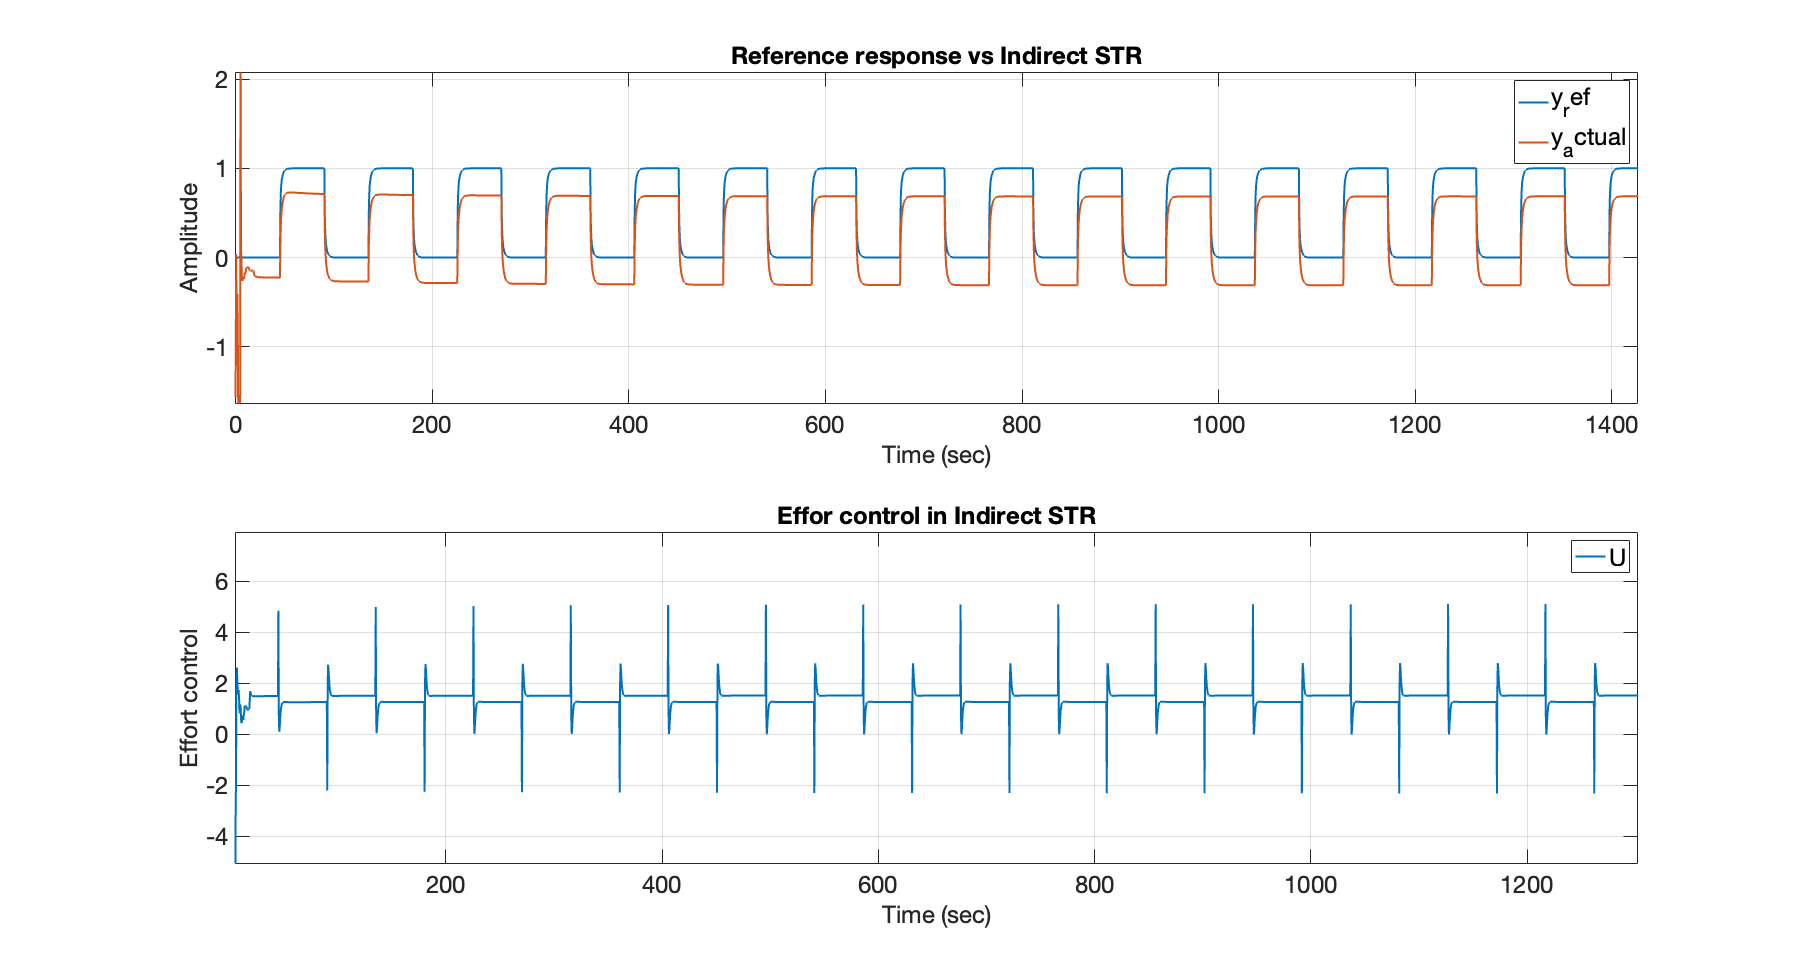
\includegraphics[width=\textwidth]{images/str81.png}
	\caption{Output with disturbance}
	\label{fig:str81}
\end{figure}

\begin{figure}
	\centering
	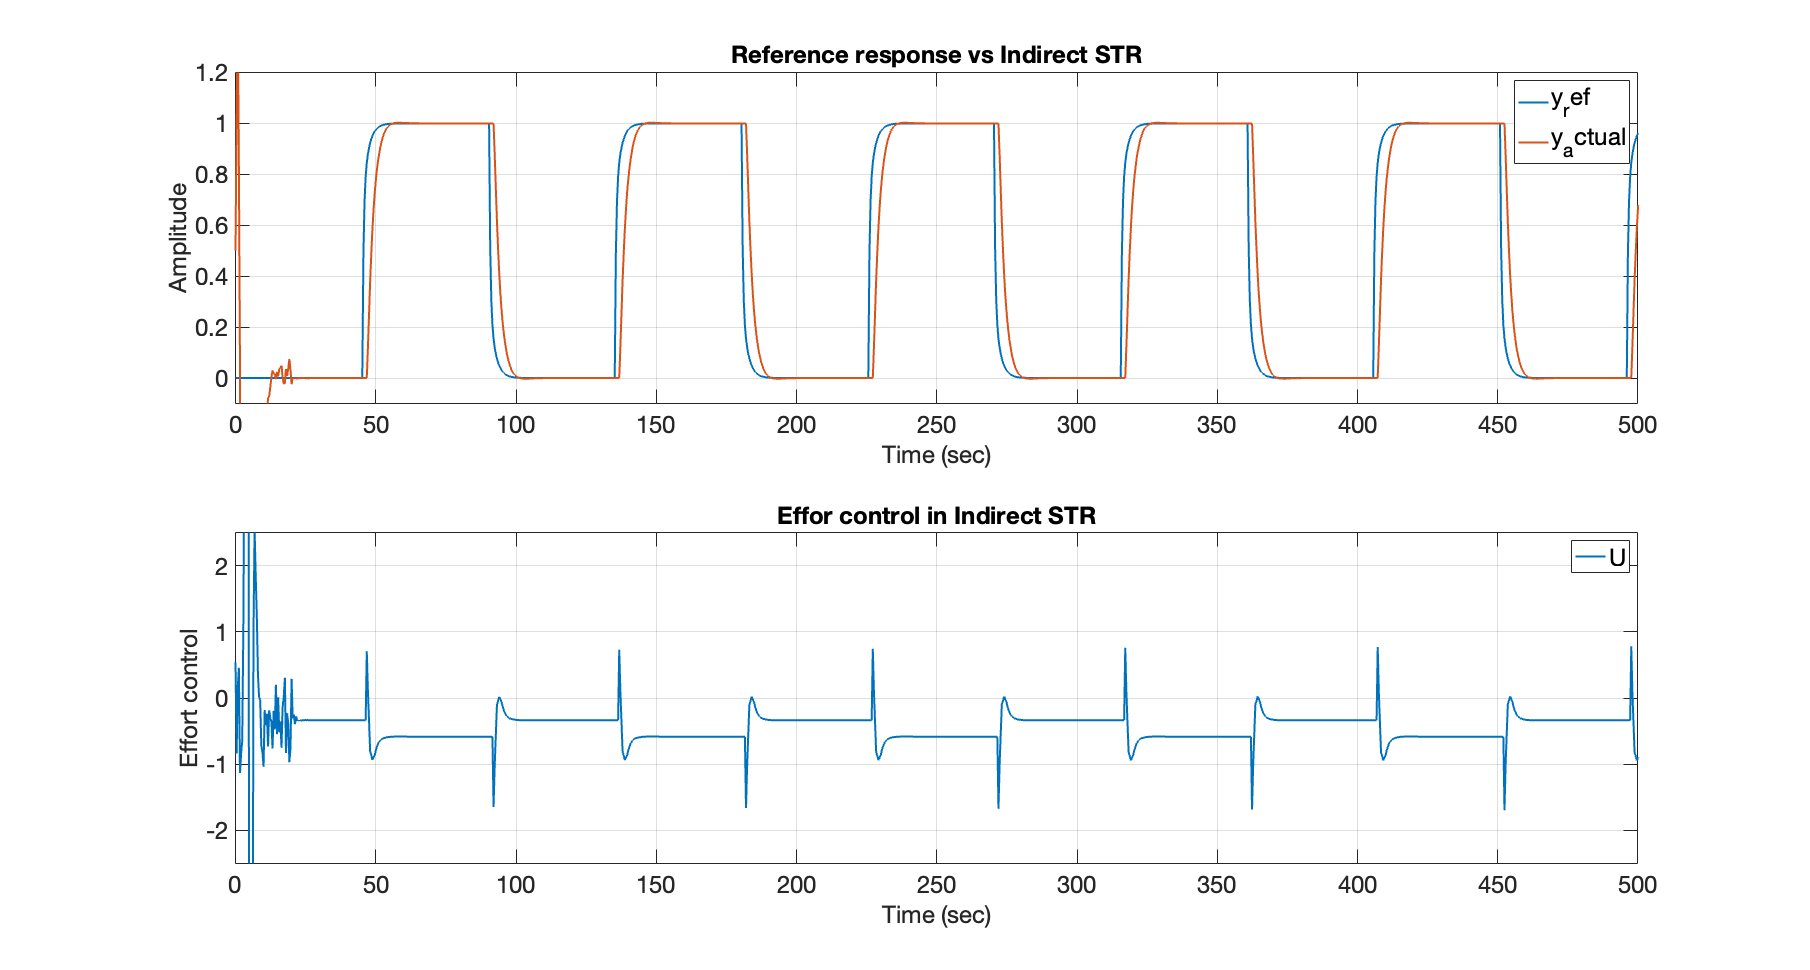
\includegraphics[width=\textwidth]{images/str82.png}
	\caption{Fixing the disturbance}
	\label{fig:str82}
\end{figure}

\begin{figure}
	\centering
	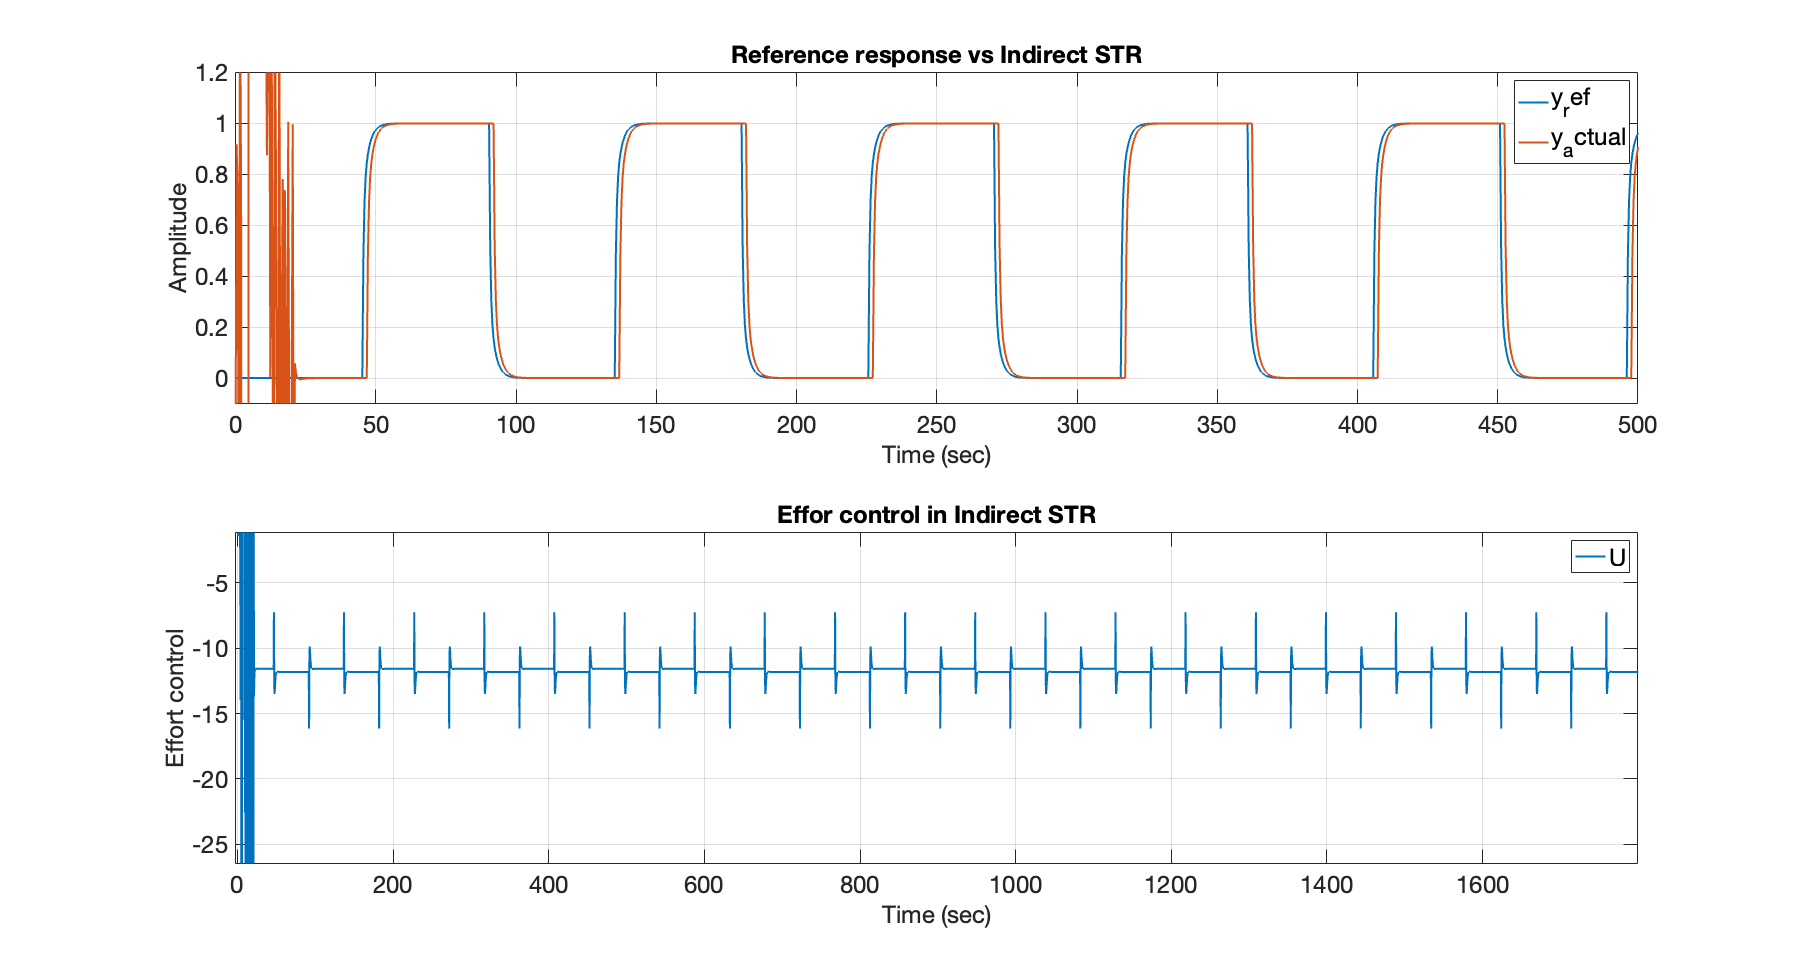
\includegraphics[width=\textwidth]{images/str83.png}
	\caption{Integral windup}
	\label{fig:str83}
\end{figure}

\begin{figure}
	\centering
	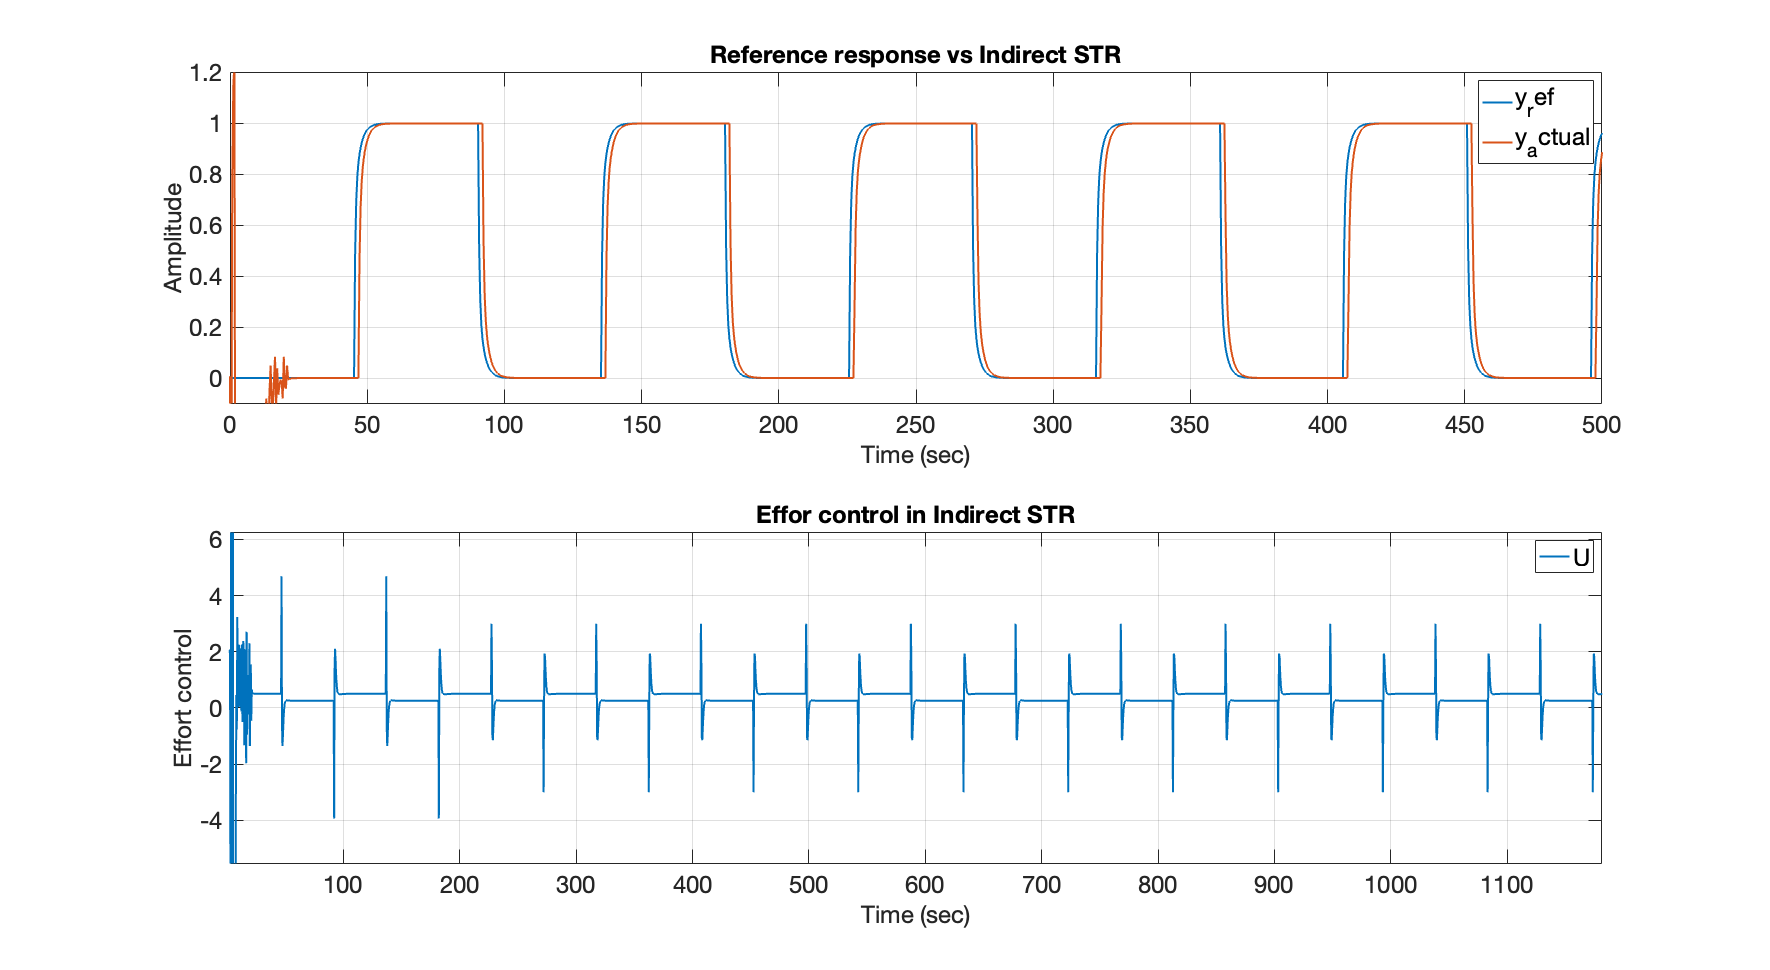
\includegraphics[width=\textwidth]{images/str84.png}
	\caption{Integral windup fix}
	\label{fig:str84}
\end{figure}

\begin{figure}
	\centering
	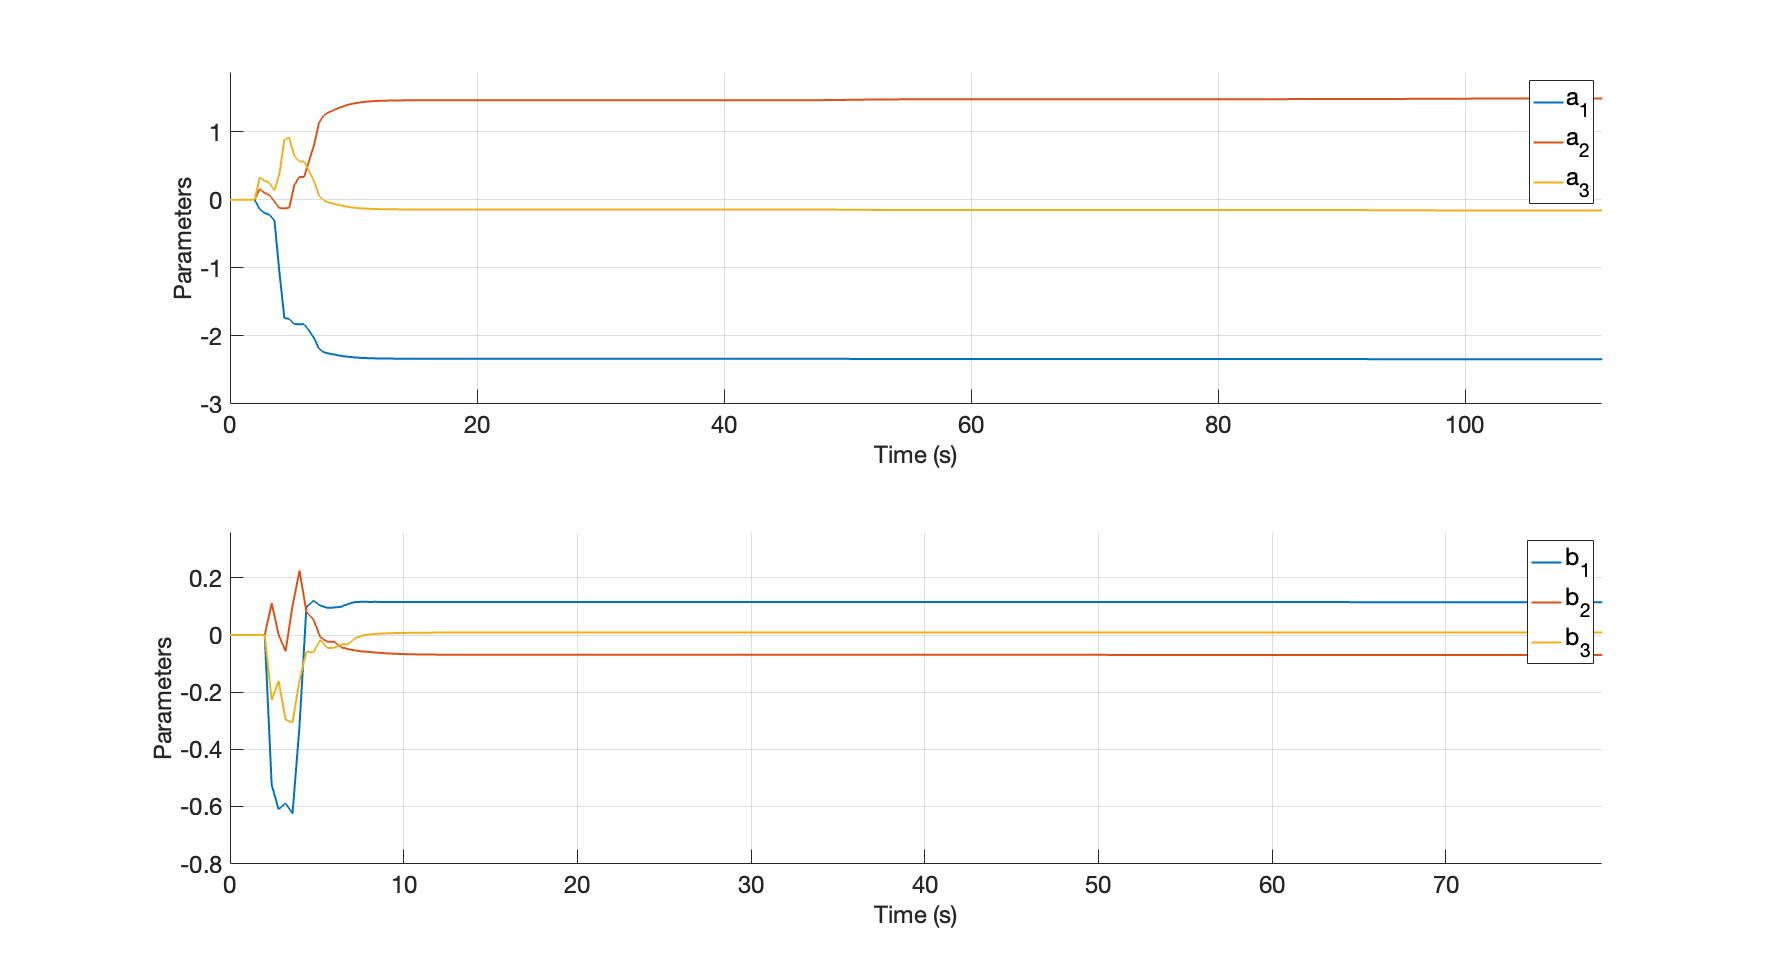
\includegraphics[width=\textwidth]{images/str85.png}
	\caption{System parameters with integral windup fix}
	\label{fig:str85}
\end{figure}

The code  for this section is available at \lstinline|assignment2/part2/STR1_indirect.m|. By changing the $distrubance=0$ to $1$ we can introduce disturbance to the system. Variables $distrubance\_fix$ and $integral\_fix$ are used to enable respective system fixes. $vlimit$ is used to limit the control output when fixing integral windup.


